\documentclass[twoside]{article}
\usepackage{amsmath,amssymb,amsthm,graphicx}
\usepackage{epsfig}
\usepackage[authoryear]{natbib}

\newcommand{\reals}{\mathbf{R}}
\newcommand{\integers}{\mathbf{Z}}
\newcommand{\naturals}{\mathbf{N}}
\newcommand{\rationals}{\mathbf{Q}}

% Caligraphic alphabet
\newcommand{\calr}{\mathcal{R}} % only because \cr already taken
\newcommand{\ca}{\mathcal{A}} \newcommand{\cb}{\mathcal{B}} \newcommand{\cc}{\mathcal{C}} \newcommand{\cd}{\mathcal{D}} \newcommand{\ce}{\mathcal{E}} \newcommand{\cf}{\mathcal{F}} \newcommand{\cg}{\mathcal{G}} \newcommand{\ch}{\mathcal{H}} \newcommand{\ci}{\mathcal{I}} \newcommand{\cj}{\mathcal{J}} \newcommand{\ck}{\mathcal{K}} \newcommand{\cl}{\mathcal{L}} \newcommand{\cm}{\mathcal{M}} \newcommand{\cn}{\mathcal{N}} \newcommand{\co}{\mathcal{O}} \newcommand{\cp}{\mathcal{P}} \newcommand{\cq}{\mathcal{Q}} \newcommand{\cs}{\mathcal{S}} \newcommand{\ct}{\mathcal{T}} \newcommand{\cu}{\mathcal{U}} \newcommand{\cv}{\mathcal{V}} \newcommand{\cw}{\mathcal{W}} \newcommand{\cx}{\mathcal{X}} \newcommand{\cy}{\mathcal{Y}} \newcommand{\cz}{\mathcal{Z}}

\newcommand{\ind}[1]{1_{#1}} % Indicator function
\newcommand{\pr}{P} % Generic probability
\newcommand{\ex}{E} % Generic expectation
\newcommand{\var}{\textrm{Var}}
\newcommand{\cov}{\textrm{Cov}}
\newcommand{\sgn}{\textrm{sgn}}
\newcommand{\sign}{\textrm{sign}}
\newcommand{\kl}{\textrm{KL}} 

\newcommand{\law}{\mathcal{L}}  % \law{X}, the measure associated with r.v. X
\newcommand{\normal}{N} % for normal distribution (can probably skip this)
\newcommand{\eps}{\varepsilon}

% Convergence
\newcommand{\convd}{\stackrel{d}{\longrightarrow}} % convergence in distribution/law/measure
\newcommand{\convp}{\stackrel{P}{\longrightarrow}} % convergence in probability
\newcommand{\convas}{\stackrel{\textrm{a.s.}}{\longrightarrow}} % convergence almost surely

\newcommand{\eqd}{\stackrel{d}{=}} % equal in distribution/law/measure
\newcommand{\argmax}{\textrm{argmax}}
\newcommand{\argmin}{\textrm{argmin}}
\newcommand{\conv}{\textrm{conv}} % for denoting the convex hull

% Theorem-like declarations
\theoremstyle{plain}
\newtheorem{theorem}{Theorem}
\newtheorem{corollary}[theorem]{Corollary}
\newtheorem{lemma}[theorem]{Lemma}

\theoremstyle{definition}
\newtheorem{definition}[theorem]{Definition}
\newtheorem{example}[theorem]{Example}

\theoremstyle{remark}
\newtheorem{remark}[theorem]{Remark}



\setlength{\oddsidemargin}{0.25 in}
\setlength{\evensidemargin}{-0.25 in}
\setlength{\topmargin}{-0.6 in}
\setlength{\textwidth}{6.5 in}
\setlength{\textheight}{8.5 in}
\setlength{\headsep}{0.75 in}
\setlength{\parindent}{0 in}
\setlength{\parskip}{0.1 in}

\newcommand{\lecture}[4]{
   \pagestyle{myheadings}
   \thispagestyle{plain}
   \newpage
   \setcounter{page}{1}
   \noindent
   \begin{center}
   \framebox{
      \vbox{\vspace{2mm}
    \hbox to 6.28in { {\bf Stat210A:~Theoretical Statistics \hfill Recitation Date: #4} }
       \vspace{6mm}
       \hbox to 6.28in { {\Large \hfill #1  \hfill}  }
       \vspace{6mm}
       \hbox to 6.28in { {\it Lecturer: #2 \hfill Scribe: #3} }
      \vspace{2mm}}
   }
   \end{center}
   \markboth{#1}{#1}
   \vspace*{4mm}
}

% Local Macros Put your favorite macros here that don't appear in
% stat-macros.tex.  We can eventually incorporate them into
% stat-macros.tex if they're of general use.

\begin{document}

\lecture{Recitation 1: Probability and measure}{Tamara Broderick}{K. Jarrod
Millman \& Richard Shin}{September 3, 2014}

\section{Densities (Radon-Nikodym)}

Recall that a random variable is a real-valued function on the event space.
In Figure~\ref{fig:figure1}, we have a two plots from the event space to values
of a random variable.

\begin{figure}[ht]
  \centering
  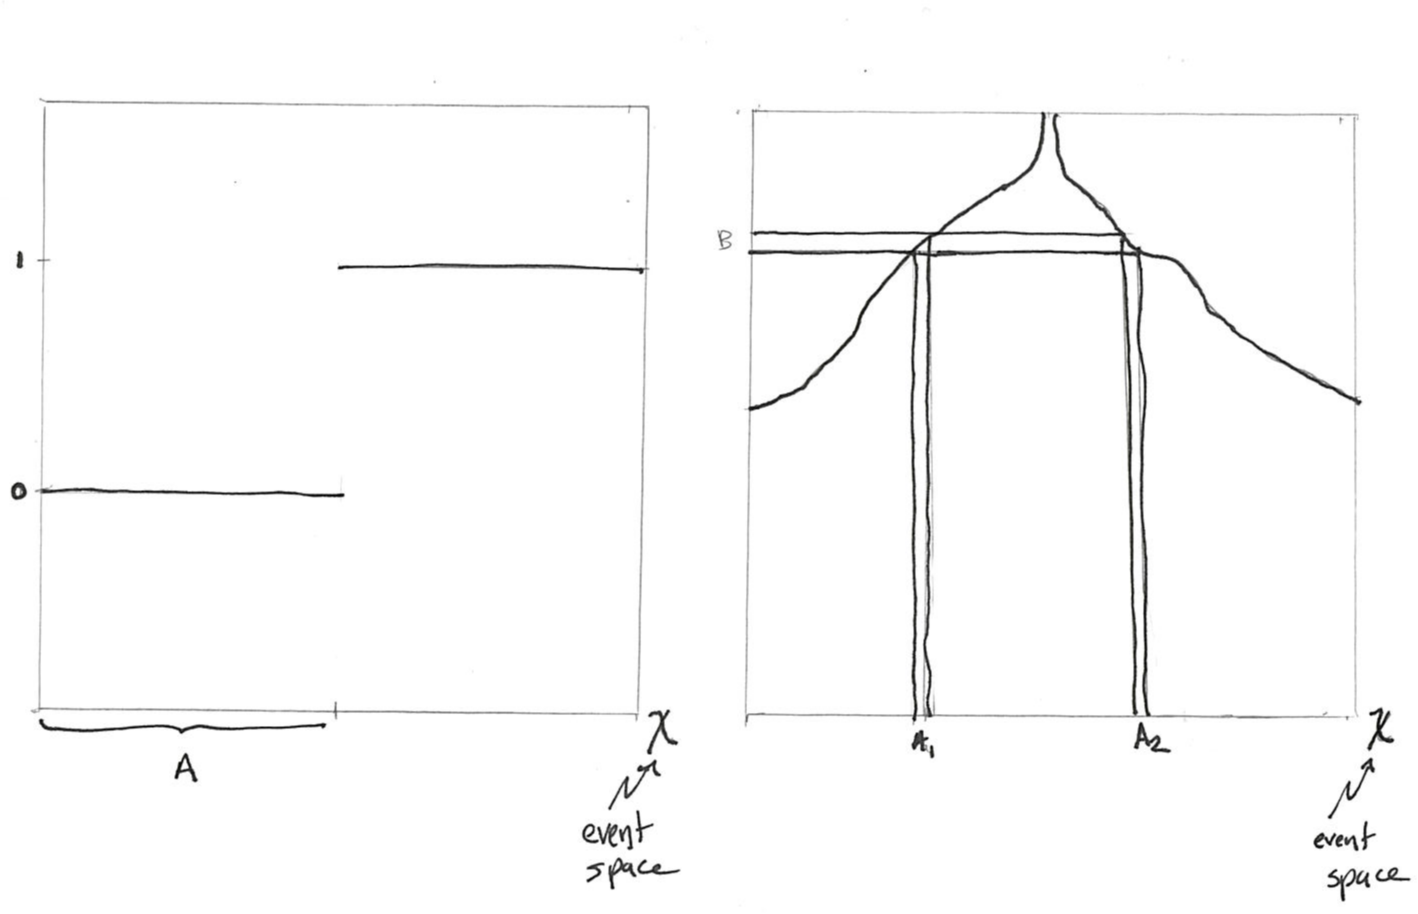
\includegraphics[width=.7\textwidth]{fig/measure-crop.pdf}
  \caption{Plots of two random variables.}
  \label{fig:figure1}
\end{figure}

To compute the probability of the random variable taking on certain values
(e.g., $0$ for the random variable in the left-hand figure above or within the
interval $B$ for the right-hand figure), we can measure the size of the
corresponding event space.  For example, in the right-hand plot above, we
have: 

\begin{align*}
\nu(X \in B) &= \mu(X^{-1}(B)) = \mu(A = A_1 \cup A_2) = \mu(A)
\end{align*}

To make this notion more precise, we first define what we mean by ``measure
the size".

\begin{definition}\label{def:measure}\citep[Def. 1.4, p.~2]{keener}
  Let $\mathcal A$ be a $\sigma$-field on a set $\mathcal X$.  A real-valued function
  $\mu$ on $\mathcal A$ is called a measure if it is non-negative and countably additive:
  \begin{enumerate}
    \item  $\mu(A) \in [0, \infty]$ for all $A \in \mathcal A$.
    \item $\sum_{i=1}^\infty \mu(A_i) = \mu\left(\bigcup_{i=1}^\infty
      A_i\right)$ when $A_i$ are disjoint.
  \end{enumerate}
  We call the tuple $(\mathcal X, \mathcal A)$ a measurable space and
  $(\mathcal X, \mathcal A, \mu)$ a measure space.  If $\mu(\mathcal X) = 1$,
  $\mu$ is called a probability measure (or probability) and $(\mathcal X, \mathcal A, \mu)$
  a probability space.  More commonly, we denote a probability space by
  $(\Omega, \mathcal F, P)$ or following the notation in Keener $(\mathcal E, \mathcal B, P)$.
  Sets $E \in \mathcal F$ are called events, elements $\omega \in \Omega$
  are called outcomes, and $P(E)$ is called the probability of $E$.
\end{definition}

In this class, we will mostly deal with the following two measures.
\begin{example} 
 If $\mathcal X = \reals^D$, let
    \[ \mu(A) = \int_{\reals^D} \cdots \int \mathbf{1}_A(x) dx_1 \cdots dx_D. \]
  Then we call $\mu$ the \emph{Lebesgue measure} on $\reals^D$.
\end{example}
\begin{example} 
  If $\mathcal X$ is countable, let
    \[ \nu(A) = \#(A \cap \integers^D). \]
  Then we call $\mu$ the \emph{counting measure} on $\mathcal X$.
\end{example}

It will be important to compare two measures.

\begin{definition}\label{def:absolutecontinuity}\citep[Def. 1.9, p.~7]{keener}
  Let $\mu$ and $\nu$ be measures on a $\sigma$-field $\mathcal A$ of the
  set $\mathcal X$. Then we say that $\nu$ is \emph{absolutely continuous} with
  respect to $\mu$, written $\nu \ll \mu$, if
  $\mu(A) = 0$ implies $\nu(A) = 0$.
\end{definition}
If $\nu \ll \mu$, we also say that $\mu$ dominates $\nu$.

\begin{example}  Let $\mu$ be the Lebesgue measure on $\reals$ and $\nu$ the counting
  measure on $\integers$.  Then
  \begin{align*}
    \mu(\{1\}) &= 0 \quad \nu(\{1\}) = 1 \\
    \mu((0, 1)) &= 1 \quad \nu((0, 1)) = 0
  \end{align*}
  Hence the Lebesgue measure and the counting measure are not absolutely continuous
  with respect to each other.
\end{example}

\begin{theorem}[Radon-Nikodym]\citep[Def. 1.10, p.~7]{keener}
  If a $\sigma$-finite measure $\nu$ is absolutely continuous with respect to a
  $\sigma$-finite measure $\mu$, then there exists an essentially unique\footnote{If $h$ is
  another non-negative function that satisfies the conditions of the Radon-Nikodym theorem,
  then $h=f$ a.e. $\mu$.} non-negative function $f$
  (sometimes denoted $\frac{d\nu}{d\mu}$) such that
  \[\nu(A) = \int_A f d\mu = \int_X f \mathbf{1}_A d\mu.\]
\end{theorem}

We will often call $f$ (or $\frac{d\nu}{d\mu}$) the Radon-Nikodym density (or
derivative).  The use of this notation and language comes from the fact that
$f$ concerns a change of measure in an integral in a similar way that the
standard derivative is used in a change of variable in an integral in classical
calculus. 

\begin{example}
  If $\mu \ll \text{Lebesgue}$, then $\mu(A) = \int_A p(x) dx$.  If $\nu(A) =
  1$, then $p(x)$ is called a probability density function.
\end{example}

\begin{example}
  If $\nu$ is absolutely continuous with respect to the counting measure. Then $\nu(A)
  = \sum_{\{m\} \in A} P(m)$.  If $\nu(X) = 1$, then $p$ is a ``probability mass
  function" (e.g., Poisson).
\end{example}

For $\mu(A)$, we have
\begin{align*}
   \int \mathbf{1}_A(x) \mu(dx) &:= \mu(A) \\
   \int a \mathbf{1}_A(x) \mu(Dx) &:= \int f d\mu,\ f = a \mathbf{1}_A \\
   \int \sum_{i=1}^n a_i \mathbf{1}_{A_i}(x) \mu(dx) &:= \int f d\mu,\ f = \sum
   a_i \mathbf{1}_{A_i}
\end{align*}

An important application of the Radon-Nikodym derivative, which we will see
again later in the course, is in the non-symmetric measure of the information
lost when using $\nu$ to approximate $\mu$.

\begin{definition}
  If  $\mu$ to $\nu$ are measures on the same measurable space and
  $\mu \ll \nu$, then the \emph{Kullback-Leibler divergence} from
  $\mu$ to $\nu$ is
  \[ D_{KL}(\mu || \nu) = \int_\chi \log \frac{d\mu}{d\nu} d\mu. \]
\end{definition}

\section{Conditional distributions (Tower Property)}

Recall the definition of conditional probabilities from elementary probability
classes.

\begin{definition}
  Let $(\Omega, \mathcal F, P)$ be a probability space with events $A$ and $B$
  such that $P(B) \neq 0$.  Then the conditional probability $P(A|B)$ of $A$
  given $B$ is defined as 
  \begin{align*}
    P(A | B) &= \frac{P(A \cap B)}{P(B)} 
  \end{align*}
\end{definition}

This definition is intuitively appealing and corresponds well with the
frequency interpretation of probability.

\begin{example}
  For discrete random variables $X$ and $Y$,
  \begin{align*}
    P(Y = y | X = x) = \frac{P(Y = y, X = x)}{P(X = x)}
  \end{align*}
\end{example}

For our purposes, it is desirable to extend the definition to allow for
the case that $P(B) = 0$.  For instance, if $B$ is the event that a
continuous random variable takes a fixed value.  

\begin{align*}
  P(Y = y) \\
  \ex[f(Y)] &= \sum_y f(y) P(Y = y) \\
  \ex[f(X, Y) | X = x] &= \sum_y f(x, y) P(Y = y | X = x)
\end{align*}
The last line is a conditional expectation.

\begin{theorem}[Tower property]
\begin{align*}
  \ex[Y | X] = \ex[\ex[Y | X, W] | X]
\end{align*}
\end{theorem}
\begin{proof}
  Here, $\ex[Y | X, W]$ is a function of $X, W$. 

  \begin{align*}
    \ex[\ex[Y | X, W] | X] &= \sum_{\tilde{x}, w} P(X = \tilde{x}, W = w | X = x)
    \cdot \left[ \sum_y yP(Y = y | X = x, W = w)\right] \\
    &= \sum_y y \sum_w \frac{P(Y = y, X = x, W = w)}{P(X = x, W = w)}  \frac{P(X =
    x, W = w)}{P(X = x)} \\
    &= \sum_y y P(Y = y | X = x)
  \end{align*}
\end{proof}
\begin{corollary}[Law of total probability]
  \[\ex[Y] = \ex[\ex[Y | W]]\]
\end{corollary}

\begin{example}
30\% of households have one child, 50\% have two children, and 20\% have
three children. What is the expected number of boys in households?
\begin{align*}
  X &= \text{\# of boys in a household} \\
  Y &= \text{\# of children in a household} \\
  \ex[X] &= \ex[\ex[X | Y]]= 0.3 \cdot 1 \cdot \frac{1}{2} + 0.5 \cdot 2 \cdot 
  \frac{1}{2} + 0.2 \cdot 3 \cdot \frac{1}{2}
\end{align*}
\end{example}

\section{Exchanging things with integration (Dominated Convergence)}

Often we will want to exchange the order of integration and another operation.
In particular, we will be interested in exchanging the order of operations with
integration and the following operations:
\begin{enumerate}
  \item other integrals
    \begin{align*}
      \int_t \int_x f(t, x) \mu(dx) \nu(dt) = \int_x \int_t f(t, x) \nu(dt) \mu(dx),
    \end{align*}
  \item limits
    \begin{align*}
      \lim_{n \rightarrow \infty} \int_x f_n(x) \mu(dx) = \int_x \left[
    \lim_{n \rightarrow \infty} f_n(x) \right] \mu(dx),
    \end{align*}
  \item and derivatives
    \begin{align*}
      \frac{\partial}{\partial t} \int_x f(t, x) \mu(dx) = \int_x
    \left[\frac{\partial}{\partial t} f(t, x)\right] \mu(dx).
    \end{align*}
\end{enumerate}

Before the stating the conditions need for the exchanging the order of integration,
we need the following definition.
\begin{definition} Let $(\mathcal X, \mathcal A, \mu)$ and $(\mathcal Y, \mathcal B, \nu)$
  be measure spaces.  Then the unique \emph{product measure} $\mu \times \nu$ on
  the measurable space $(\mathcal X \times \mathcal Y, \mathcal A \vee \mathcal B)$ satisfies
  \begin{align*}
    (\mu \times \nu)(A\times B) &= \mu(A)\nu(B)
  \end{align*}
  for all $A \in  \mathcal A$ and $B \in \mathcal B$.
\end{definition}
Note that $\mathcal A \vee \mathcal B$ is taken to be the smallest $\sigma$-field on
$\mathcal X \times \mathcal Y$.
\begin{theorem}[Fubini-Tonelli]\citep[Theorem 1.7, p.~13]{keener}
  Let $(\mathcal X, \mathcal A, \mu)$ and $(\mathcal Y, \mathcal B, \nu)$
  be measure spaces.  If either (Tonelli's condition) $f \geq 0$ or (Fubini's
  condition) $\int |f| d(\mu \times \nu) < \infty$  hold, then
  \begin{align*}
    \int_{X\times Y} f d(\mu \times \nu) &= \int_Y \int_X f(x, y) d\mu(x) d\nu(y) \\
    &= \int_X \int_Y f(x, y) d\nu(y) d\mu(x).
  \end{align*}
\end{theorem}

Moving the limit under the integral is primarily of interest because if we can
do that, we can move differentiation under the integral since it is a special
case of a limit.  If the domain of integration is finite, then we can exchange
differentiation with the integral by Leibniz' rule.  However, when the domain
of integration isn't finite things become more complicated as illustrated by
the following example.

\begin{example}
Consider the sequence of functions $f_n(x) = \mathbf{1}_{(n, n+1)}(x)$ for all
$x \in \reals$.  Then
\begin{align*}
  \lim_{n \rightarrow \infty} f_n(x) &= 0 \quad \text{for all $x$, but}\\
  \lim_{n \rightarrow \infty} \int f_n(x) dx &= 1.
\end{align*}
\end{example}

The following theorem gives conditions under which we can move such a limit
past an integral.

\begin{theorem}[Dominated convergence]\citep[Theorem 2.5, p.~29]{keener}
  Let ${f_n}$ be a sequence of real-valued measurable functions on a
  measure space $(\mathcal X, \mathcal A, \mu)$ such that there is some
  $g$ with $|f_n| \le g$ (a.e. $\mu$) for all $n$.  If $\int g d\mu < \infty$
  and $\lim_{n \rightarrow \infty} f_n(x) = f(x)$ for a.e. $x$ under $\mu$,
  then
  \begin{align*}
    \lim_{n \rightarrow \infty} \int f_n(x) \mu(dx) &= \int
      \left(\lim_{n \rightarrow \infty} f_n(x) \right) \mu(dx) \\
       &= \int f(x) \mu(dx) \\
       &= \int f d\mu.
  \end{align*} 
\end{theorem}

\begin{example}[from class on Tuesday]
Recall that the 1-parameter exponential family in canonical form is given by
\begin{align*}
  p_\eta(x) &= e^{\eta T(x) - A(\eta)} h(x) \quad \text{for }
  \eta \in \text{canonical parameter space}
\end{align*}
where $A(\eta)$ is called the log-partition function (i.e., the
logarithm of the normalizing constant).  That is,
\begin{align*}
  e^{A(\eta)} &:= \int e^{\eta T(x)} h(x) \mu(dx).
\end{align*}
Taking the derivative with respect to $\eta$ of the right-hand side yields
\begin{align}
  \frac{\partial}{\partial \eta} e^{A(\eta)} &= e^{A(\eta)}
    \frac{\partial}{\partial \eta}A(\eta)
\end{align}
While taking the derivative with respect to $\eta$ of the left-hand side
yields
\begin{align}
  \frac{\partial}{\partial \eta} \int e^{\eta T(x)} h(x) \mu(dx)
  &= \lim_{n \rightarrow \infty} \left[ \int e^{(\eta + c/n)T(x)} h(x) \mu(dx) -
  \int e^{(\eta + 0)T(x)} h(x) \mu(dx) \right]/ \frac{c}{n} \notag\\
  &= \lim_{n \rightarrow \infty} \int \underbrace{e^{\eta T(x)} \left[
  \frac{e^{(c/n)T(x)} - e^{0 \cdot T(x)}}{c/n} \right] h(x)}_{f_n(x)} \mu(dx)
\end{align}
Assume there exists a $g$ such that $|f_n(x)| \le g(x)$ and
$\int g(x) \mu(dx) < \infty$, so dominated convergence.
\begin{align*}
  &= \int \frac{\partial}{\partial \eta} \left[e^{\eta T(x)}\right] h(x) \mu(dx) \\
  &= \int T(x) e^{\eta T(x)} h(x) \mu(dx)  \\
  &= e^{A(\eta)} \ex[T(X)] \\
  &\Rightarrow \frac{\partial}{\partial \eta} A(\eta) = \ex[T(X)]
\end{align*}
\end{example}


\bibliographystyle{apalike}
\bibliography{stat}

\end{document}
